% REMEMBER: You must not plagiarise anything in your report. Be extremely careful.

\documentclass{l4proj}

    
%
% put any additional packages here
%

\begin{document}

%==============================================================================
%% METADATA
\title{Emulating Glasgow's First Computer}
\author{Gerard Ward}
\date{September 14, 2018}

\maketitle

%==============================================================================
%% ABSTRACT
\begin{abstract}
    Every abstract follows a similar pattern. Motivate; set aims; describe work; explain results.
    \vskip 0.5em
    The English Electric DEUCE was one of the first commercially available computers in the world,
    but in modern times, there are limited resources available to learn more about it. The aim of
    this project was to create an emulator of the DEUCE, to provide people with a way of learning
    how one of the world's earliest computers functions. Written as a web application, this emulator
    allows users to operate the DEUCE as if they were using an original, but through a modern software
    solution. In the end, the project captured most of the functionality of the original DEUCE.
    
\end{abstract}

%==============================================================================

% EDUCATION REUSE CONSENT FORM
% If you consent to your project being shown to future students for educational purposes
% then insert your name and the date below to  sign the education use form that appears in the front of the document. 
% You must explicitly give consent if you wish to do so.
% If you sign, your project may be included in the Hall of Fame if it scores particularly highly.
%
% Please note that you are under no obligation to sign 
% this declaration, but doing so would help future students.
%
%\def\consentname {My Name} % your full name
%\def\consentdate {20 March 2018} % the date you agree
%
\educationalconsent


%==============================================================================
\tableofcontents

%==============================================================================
%% Notes on formatting
%==============================================================================
% The first page, abstract and table of contents are numbered using Roman numerals and are not
% included in the page count. 
%
% From now on pages are numbered
% using Arabic numerals. Therefore, immediately after the first call to \chapter we need the call
% \pagenumbering{arabic} and this should be called once only in the document. 
%
% The first Chapter should then be on page 1. You are allowed 40 pages for a 40 credit project and 20 pages for a 
% 20 credit report. This includes everything numbered in Arabic numerals (excluding front matter) up
% to but excluding the appendices and bibliography.
%
% You must not alter text size (it is currently 10pt) or alter margins or spacing.
%
%
%==================================================================================================================================
%
% IMPORTANT
% The chapter headings here are **suggestions**. You don't have to follow this model if
% it doesn't fit your project. Every project should have an introduction and conclusion,
% however. 
%
%==================================================================================================================================
\chapter{Introduction}

% reset page numbering. Don't remove this!
\pagenumbering{arabic} 

This chapter states the motivations and aims behind this project, as well as summarising the
contents of the rest of this dissertation. The DEUCE emulator built for this project allows
users to operate a web application version of the English Electric DEUCE. The significance of creating
this emulator will be explained in this chapter.

\section{Motivation}

In 1951, the English Electric company began building models of the Digital Electronic Universal Computing Engine, also known as the DEUCE. This computer was based on Alan Turing's Pilot ACE computer but improved on the ACE in several ways, namely by improving upon the speed and reliability of the ACE, adding further storage and adding a large program and subroutine library. Due to these improvements, the DEUCE was considered a commercial success: in total, approximately 33 DEUCEs were created. These were mainly installed at governmental departments, aircraft design facilities and universities. Therefore, as an early, commercially successful stored program computer, the DEUCE has a hugely important part in the history of Computing Science.

Among the universities that installed a DEUCE was the University of Glasgow. In 1957, the university established Scotland's first computing lab and chose Dennis Gilles as its initial director. As director, Gilles was responsible for advising the university to order its first computer and so in 1958, the DEUCE became the first electric computer at a Scottish university. In addition to holding an important place in the history of Computing, the DEUCE also holds an important place in recent Scottish academic history.

However, in spite of the DEUCE's importance as an early electric computer, there remain limited resources available on the DEUCE. With all of the machines having stopped being in use since approximately the late 1960s, there are no DEUCEs left to use in the world today. At the University of Glasgow, the only remaining piece of the DEUCE installed there is one of the mercury delay lines. For this reason, it would be beneficial if there were a modern way of allowing people to operate a DEUCE in order to learn more about an important part of Computing Science history, and also to learn how to operate an example of an early computer.

Therefore, a solution to this problem is to create a modern emulator of the DEUCE. In doing so, this would allow for the DEUCE's legacy to continue.

\section{Aims}

For this project, the key aim is to create a functioning emulator of the DEUCE. The emulator should replicate the behaviour of the original DEUCE, using the same input, processing and output methods. When completed, the emulator should allow the user to run programs on it, as if it were the original DEUCE computer. It should also replicate the user interface of the DEUCE. After the emulator has been created, it should be evaluated against the DEUCE to discover if it can run programs written for the original computer.

\section{Summary}

The purpose of this chapter was to introduce they key motivations behind the project and what the aims of the project should be. The rest of this dissertation will be structured as follows:

\begin{itemize}
	\item Chapter 2 will examine the background research carried out on how the DEUCE functioned. It will also examine similar early computer emulators and look into what made these emulators examples of good or bad emulators.
	\item Chapter 3 will examine the requirements gathering process for the emulator and the choices behind the target platform chosen for the project.
	\item Chapter 4 will examine the initial design choices made for the emulator and the decisions which informed the design of both the graphical and system design of the computer.
	\item Chapter 5 will discuss the implementation process of the project and how the frontend and backend of the project was implemented.
	\item Chapter 6 will examine how the emulator was evaluated against the original DEUCE, to discover how successful it was in emulating its behaviour.
	\item Chapter 7 will reflect on possible future steps for the project and what could have been improved about the emulator. 
\end{itemize}

%==================================================================================================================================
\chapter{Background}
This chapter discusses background research carried out on the DEUCE and on the creation of emulators.
\begin{figure}[h]
	\centering
	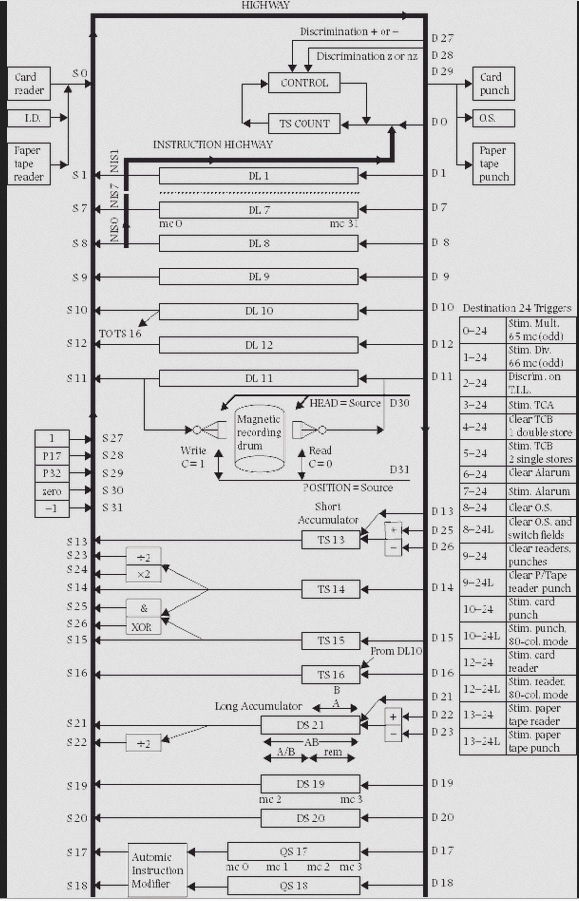
\includegraphics[width=0.5\linewidth]{images/deuce-arch.jpg} 
	\caption{Architecture diagram of the DEUCE.}
	\label{fig:arch}
\end{figure}

\section{Learning how the DEUCE functions}
Firstly, it was important to learn how the DEUCE functioned as a computer. The architecture of the DEUCE is shown in Figure 2.1. As an early computer, it is extremely different to modern computers in several ways. For example, for input, the instructions read in by the DEUCE were essentially a series of move instructions from a memory source to a memory destination. Each instruction was a 32-bit binary word. Instructions could be read in either via a card reader, which read in lines of instructions on special cards, or through the Input Staticiser, a special row of switches which allowed for single word input. Several special source and memory locations specified special functions, such as arithmetic functions, discrimination functions etc., and through using these special memory locations, the computer could be coded to run programs.

The DEUCE stored instructions in delay lines and registers. It consisted of:
\begin{itemize}
	\item 32 mercury delay lines, each storing 32 words.
	\item 4 Temporary Store registers, each storing 1 word.
	\item 3 Double Store registers, each storing 2 words.
	\item 2 Quadruples Store registers, each storing 4 words.
\end{itemize}	
For output, the DEUCE could display information through the Output Staticiser, which was a row of lights that could display a single 32-bit word, or through a screen which could display a matrix of bits.

The complex mechanics of the DEUCE meant that the architecture of the computer had to be studied carefully in order to fully understand how to emulate its behaviour.

\section{Comparison of early computer emulators}
To gain a better understanding of how early computers worked, several emulators of other early computers were used. This gave good insight into how similar early computers functioned and explore the design choices made by the creators of these emulators.
\subsection{Pilot ACE Emulator} 
\begin{figure}[h!]
	\centering
	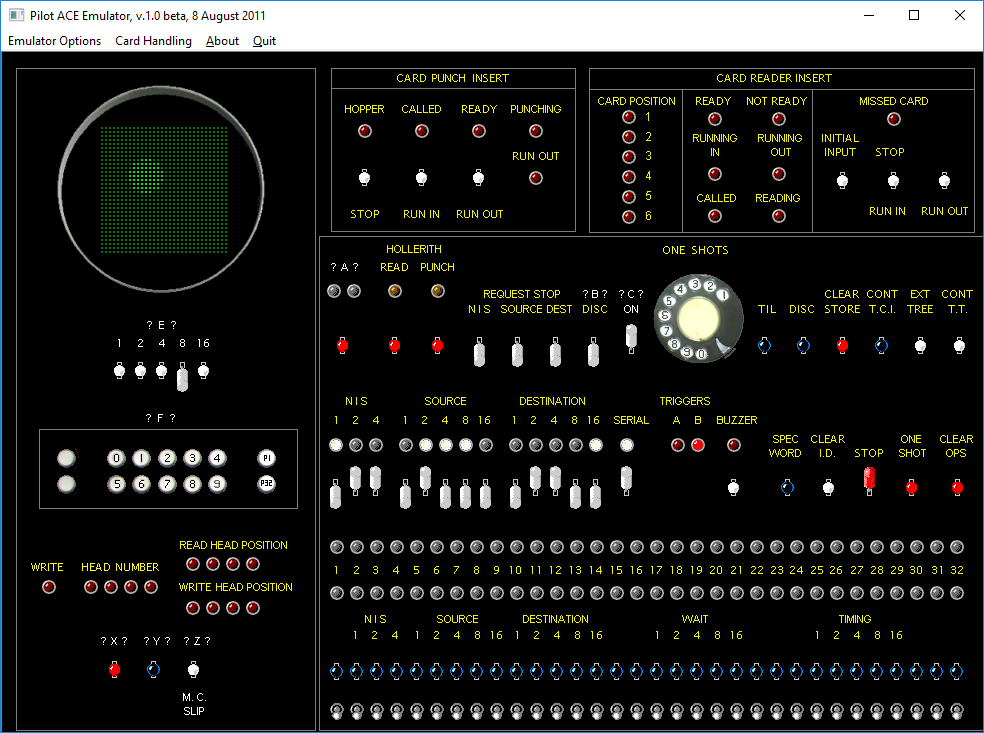
\includegraphics[width=0.7\linewidth]{images/ace-emulator}
	\caption{Pilot ACE Emulator from http://www.pilotaceonline.com/index.html}
	\label{fig:ace}
\end{figure}
The Pilot ACE was one of the earliest stored-program computers and was based on a design by Alan Turing, running its first program in 1950. The DEUCE was a commercial version of this machine, so there are several similarities between the two computers. For example, both machines can read input from a Hollerith card reader or from the input dynamiciser keys on the front panel of the machine. The main memory of the Pilot ACE consisted of 11 32-bit delay lines, 5 32-bit temporary stores and 2 64-bit double stores.

This emulator is a very faithful recreation of the original Pilot ACE. The panel is a replica of the original panel of the Pilot ACE. To recreate some of the physical actions of operating tnhe Pilot ACE, such as inserting a card into the card reader, the author has instead provided a toolbar which allows some of these features to be carried out.

Therefore, the Pilot ACE emulator is a very useful model on which to base a DEUCE emulator. Given the similarities in how the Pilot ACE and DEUCE computers functioned, this emulator provided some very good ideas about how to implement a DEUCE emulator. As the DEUCE was a commercial version of this machine, many of the features present in this emulator can be reused in a DEUCE emulator, such as the input dynamiciser and single shot key. While the GUI is an accurate representation of the original Pilot ACE interface, several of the features of the original Pilot ACE appear unknown to the author. For example, the purposes of the keys surrounded by question marks, such as ? E ?, are unknown to the creator. Overall, it would be worthwhile to base several features of a DEUCE emulator on this emulator.


\subsection{The EDSAC Simulator}
\begin{figure}[h!]
	\centering
	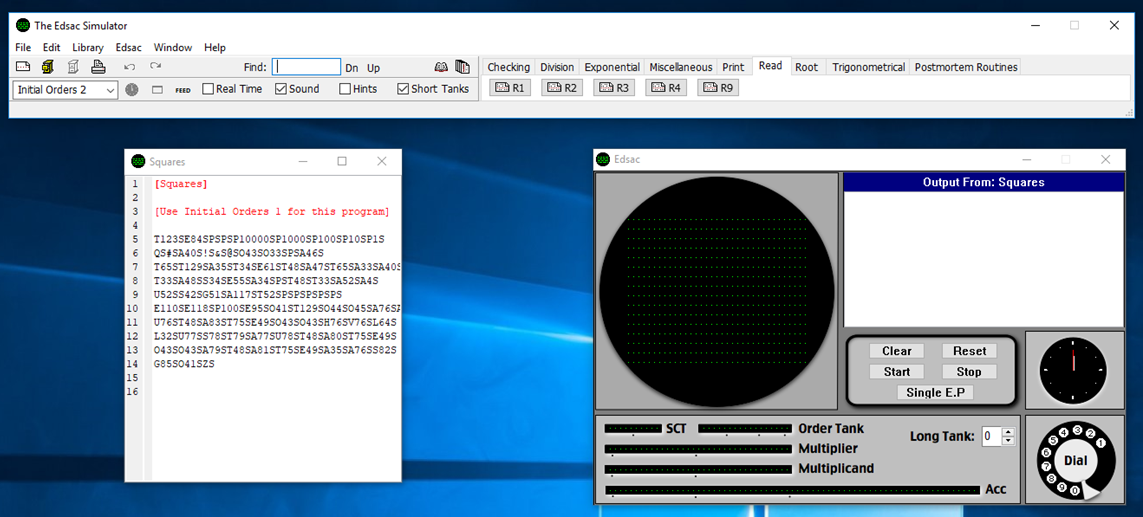
\includegraphics[width=\linewidth]{images/edsac-emu}
	\caption{EDSAC Simulator from https://www.dcs.warwick.ac.uk/~edsac/}
	\label{fig:edsac}
\end{figure}

Like the Pilot ACE and the DEUCE, the EDSAC was another early stored program computer. Running its first program in 1949, it used 32 mercury delay lines for main memory, each storing 32 words of 18 bits. For input, it used a paper-tape reader operating at 50 characters per second and output was achieved through a Creed teleprinter. Control can be achieved through five buttons: clear, reset, start, stop and single E.P. Single E.P functions similarly to the single shot key in the DEUCE, by allowing a program to be executed one instruction at a time. 

The EDSAC emulator has three main components: the toolbar, the program text and the simulator display. 
The toolbar allows control over the features of the EDSAC. For example, it allows files to be read in and allows the user to switch between Initial Orders 1 and Initial Orders 2. The program text provides the series of instructions to be executed for a program that is being read in. The simulator display shows the output from the programs being executed and allows control over programs through the five main control buttons.

Overall, while there are bigger differences between the DEUCE and the EDSAC than the DEUCE and the Pilot ACE, this is still a useful emulator on which to model some features of the DEUCE. Both computers share common features such as using a reader to take input from files and using delay lines for main memory. One useful feature of this emulator compared to the Pilot ACE emulator is its output display. Rather than outputting to a new file, it is useful to have a console that displays output instead. This would be a good feature to have in a DEUCE emulator, particularly one running as a web app. Therefore, while several features would need to change, there are some features of this emulator that would be useful to base a DEUCE emulator on.

\subsection{Manchester Baby Emulator}
\begin{figure}[h!]
	\centering
	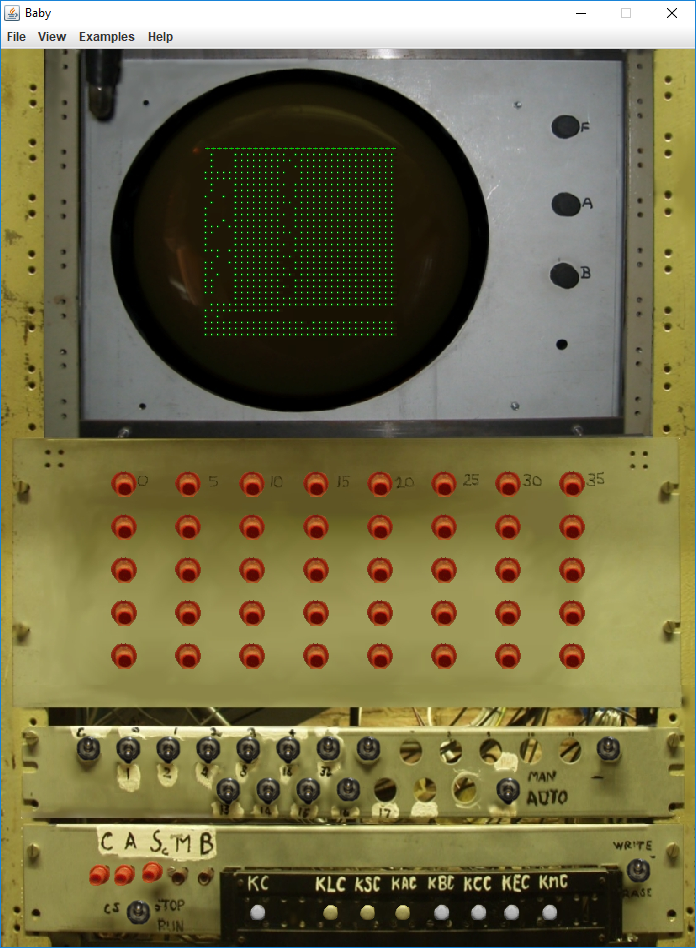
\includegraphics[width=0.5\linewidth]{images/baby-emu}
	\caption{Manchester Baby Emulator from https://www.davidsharp.com/baby/}
	\label{fig:baby}
\end{figure}

The Manchester Baby was another early computer. It was the first electronic stored program computer in the world, running its first program in 1948 before the Pilot ACE and the EDSAC. Its memory is made up of 32 store lines, each containing 32 bits. In one store line, bits 0-4 represent the operand line, i.e. the number of the line that the instruction will operate on when executed, and bits 13-15 represent the function number, which is essentially the instruction opcode.

The control of the Manchester Baby contains two values: the control instruction (CI) and the present instruction (PI). The CI contains the line number of the instruction executed previously. The PI contains the line representing the instruction currently being executed. Input can also be controlled using the switches on the front panel. Output can be displayed through the monitor above the control panel.

Regarding this emulator of the Manchester Baby, the creator chose to make it photo realistic, so it resembles the interface of the original Manchester Baby. While this is a faithful recreation, the interface feels slightly more intimidating to use than the other emulators used so far. For this reason, it would probably be better to recreate the DEUCE using a cleaner interface rather than faithfully restoring the interface as above.
The toolbar of this emulator provides control so the user can load different example programs and view the different parts of the computer, such as the store, the control, the accumulator and the disassembler. The examples tab is a useful way of loading in new programs easily so new users can quickly learn how to use the machine. It would be beneficial to replicate a feature such as this in a DEUCE emulator.

\section{Summary}
In carrying out background research, this allowed for the discovery of how the DEUCE functioned compared to modern computers and what makes for a good emulator of an early computer. Overall, the design of the DEUCE emulator for this project would be similar to the Pilot ACE emulator, as the two original computers shared much of the same design. Using this research, this allowed for the creation of formal requirements as specified in Chapter 3.

%==================================================================================================================================
\chapter{Analysis/Requirements}
This chapter examines the process of analysing how to create the DEUCE emulator. The scope of the project is discussed, as well as the requirements gathered to create the emulator.

\section{Platform selection}
The original project plan was to create a DEUCE emulator for mobile platforms, but after considering several factors concerning the feasibility of creating a mobile emulator, it was agreed instead to make a web application. Firstly, it would have been extremely difficult to recreate a faithful DEUCE emulator on mobile devices given the limitations of mobile device screen sizes. For example, the DEUCE's Input Dynamisciser was a row of 32 switches, so trying to create a good interface for this on a mobile device would have been beyond the scope of this project.

Furthermore, creating this emulator as a web application is a modern solution to making the DEUCE accessible to a wide number of people. By hosting the emulator on a website, users can access it through their web browser on any device, including desktop or mobile. Therefore, the decision to change the scope of the project early on was important in order to recreate the DEUCE as faithfully as possible.

\section{Requirements Gathering}
Requirements elicitation was an important early step in the Analysis stage of the project. This helped to define what could feasibly be completed within the scope and time frame of the project. Initial general requirements were firstly created. They are as follows:
\begin{itemize}
	\item Replicate physical features of the DEUCE, such as delay lines, card reader etc., within a modern software solution.
	\item Have a graphical user interface resembling that of the original DEUCE
	\item Allow users to interact with input switches, most likely through a pointing device.
	\item Read in programs written as "punch cards".
	\item Execute programs in the same way as the original DEUCE.
	\item Display output through representations of lights on console.
	\item Be intuitive enough for those familiar with the DEUCE to be able to operate it.	
\end{itemize}
	
While these requirements sufficed as early, broad requirements, it was necessary to then refine them and categorise them into functional and non-functional requirements.

\subsection{Functional Requirements}
The functional requirements of the project define what features DEUCE emulator should have. These were categorised into Must Have, Should Have, Could Have and Won't Have (this time) requirements, using the MoSCoW method. They are as follows:
\\
 
\textbf{\textit{Must Have:}}
\begin{itemize}
	\item A row of 32 Input Dynamiciser switches, to allow for single instruction and data input.
	\item A row of 32 Input Dynamiciser lights, to display the status of the Input Dynamiciser.
	\item A row of 32 Output Staticiser lights, to display output from instructions.
	\item A memory storage system comprised of 12 Delay Lines, 4 Temporary Stores, 3 Double Stores and 2 Quadruple Stores. These must store the following:
	\begin{itemize}
		\item Delay Lines must store 32 32-bit words each.
		\item Temporary Stores must store 1 32-bit word each.
		\item Double Stores must store 2 32-bit words each.
		\item Quadruple Stores must store 4 32-bit words each.
	\end{itemize}
	\item A clock to simulate delay line acoustic pulses, which are needed to access delay line memory.
	\item An instruction decoder that calculates the NIS, Source, Destination, Wait, Timing and Go values of an instruction.
	\item A single shot switch to execute a single instruction.
	\item A graphical user interface resembling that of the original DEUCE.
	\item A series of special Source and Destination addresses, as follows:
	\begin{itemize}
		\item Source 0 - Take user input from Input Dynamiciser.
		\item Source 23 - Divide contents of TS14 by 2 and place in selected destination address.
		\item Source 24 - Multiply contents of TS14 by 2 and place in selected destination address.
		\item Source 25 - LOGICAL AND contents of TS14 and TS15 and place in selected destination address.
		\item Source 26 - EXCLUSIVE OR contents of TS14 and TS15 and place in selected destination address.
		\item Source 27 - Place 1 (UNITY) in selected destination address.
		\item Source 28 - Place $ 2^{16} $ in selected destination address.
		\item Source 29 - Place $ 2^{31} $ in selected destination address.
		\item Source 30 - Place 0 (ZERO) in selected destination address.
		\item Source 31 - Place -1 in selected destination address.
		\item Destination 25 - Add the contents of the Source address to TS13 and store result in TS13.
		\item Destination 26 - Subtract the contents of the Source address from TS13 and store result in TS13.
		\item Destination 27 - Discriminate between positive and negative numbers.
		\item Destination 28 - Discriminate between zero and non-zero numbers.
		\item Destination 29 - Display output on Output Staticiser.
		
	\end{itemize}
\end{itemize}

\textbf{\textit{Should Have:}}
\begin{itemize}
	\item A single shot dial to execute a given number of single shots in succession.
	\item A card reader to take external input from a pre-written DEUCE program.
	\item A card punch to write programs to external files.
	\item A Clear ID switch to clear the Input Dynamiciser lights to 0.
	\item A Clear Ops switch to clear the Output Staticiser lights to 0.
	\item A Clear Store switch to clear all data held in delay line storage.
	\item A Read and Single Read switch to read in punch cards.
	\item A Punch switch to write to output files.
	\item An Initial Input switch to read a new program.
	\\
	\\
	
\end{itemize}

\textbf{\textit{Could Have:}}
\begin{itemize}
	\item A user manual to instruct users on how to operate the DEUCE.
	\item A more convenient way of viewing the current memory contents of the DEUCE. While not an original feature of the DEUCE, this could help new users to view the state of their programs.
	
\end{itemize}

\textbf{\textit{Won't Have (this time):}}
\begin{itemize}
	\item A monitor to display output. This requirement would be extremely challenging to implement within the scope of this project and so will not be included this time.
	\item A subroutine library. The original DEUCE came with a large library of subroutines to be used by DEUCE programmers but this would be too much to implement within the time frame of the project.
\end{itemize}
\subsection{Non-functional Requirements}
The non-functional requirements of the project describe how the emulator should work, rather than describing what the emulator will do. 
\begin{itemize}
	\item The emulator should be easy enough to understand how to operate for those familiar with the DEUCE.
	\item It should be intuitive so that new users can learn how to operate a DEUCE.
	\item It should be designed mainly for desktop computer users but also be available on other devices such as tablets and mobile phones.
	\item It should be maintainable so that development can be continued in future.
\end{itemize}

\section{Summary}
This chapter gives an overview of the steps taken during the Analysis stage of the development of the project. The decision to change the project scope from being a mobile development project to a web development project was highly important, as it showed the steps taken to calculate the feasibility of the project on web compared to mobile. This stage was also key in the development process as it involved the creation of formal requirements for the project. Following these requirements would prove highly important for the rest of the project.

%==================================================================================================================================
\chapter{Design}
This chapter examines the design of the DEUCE emulator. The design of the emulator can broadly be split into two parts: the system architecture and the user interface. The design of the system architecture is concerned with the logical design of the components which make up the computer, while the user interface design examines the graphical aspect of the emulator and how to present it to users.
\section{System Architecture}
Recreating the system architecture of the DEUCE entirely within software was an important step in the design process. With much of the system architecture of the original DEUCE being physical, it was necessary to consider abstract alternatives to how the system could be imitated entirely within software. The main design concepts concerning the DEUCE emulator are detailed within this section.

\subsection{Memory Storage}
The creation of the memory storage of the DEUCE emulator presented several design questions at an early stage. Firstly, the DEUCE had two levels of main memory: delay lines and registers. Access to each of these levels was different as the delay line used clock pulses to access data, whereas for Temporary Stores, access was instant. Delay lines could also hold a vast amount of words compared to registers. Furthermore, within the registers themselves, there were varying sizes between Temporary Stores, Double Stores and Quadruple Stores. Therefore, a solution was needed to represent these different levels of memory entirely within software.

An initial design solution to this problem was to create a dictionary to hold each type of storage. With keys for each type of storage, this would allow a way of accessing each level of memory entirely within software. For every key, the value pair would be an array holding the number of words each type of storage could hold. For example, keys "DL1" to "DL12" would represent the 12 Delay Lines of the DEUCE and hold an array of 32 words, while "TS13" being Temporary Store 13 could hold 1 word.

Another proposed solution to this was to simply store all levels of memory within one array of "Memory" objects. Each memory object could hold a given number of words and so could be used to represent each type of storage. The index of each type of storage would have to be tracked rather than named but given the labels of each type of storage in the architecture diagram of the original DEUCE (DL1, TS13, QS17 etc.) seen in Figure \ref{fig:arch}, it would not be difficult to do so. The number of each type of storage from the labels could be simply used as indexes within the array.

For this reason, it was decided that an array would be used over a dictionary. Ultimately, using a dictionary would overcomplicate the design of memory as software and an array would be a more efficient and effective way of keeping track of memory.
\subsection{Delay Line Architecture}
Following on from the overall design of the memory storage of the DEUCE, another large design challenge regarding the system architecture of the DEUCE emulator was the design of access to the delay lines. In early computers, delay lines provided fast access to data using mercury and acoustic pulses. With the data constantly flowing in the mercury tanks, it was necessary to keep track of where the data was in the delay lines using minor and major cycles. One minor cycle represented one pulse, while one major cycle represented how long it took for data to flow around an entire delay line. This is why DEUCE instructions feature Wait and Timing numbers, as these numbers calculate where in the delay lines certain data will be.

Within a web application version of the DEUCE, the design of the delay line storage of the DEUCE posed a problem. Without physical mercury delay line storage available to this emulator, a suitable substitute was needed to represent this behaviour. To emulate the behaviour of minor and major cycles of delay lines, it was deicded that there should be a clock to measure minor cycles. This would be designed as a counter that would increment by 1 every minor cycle. Using this counter, it would be possible to track where data was being held in each delay line. Essentially, this counter would act like a pointer to an array. This solved the design problem of using an alternative to physical delay line storage.

\subsection{Instruction Processing}
The design of how instructions would be processed in the DEUCE emulator was another challenging task. Each memory location in the DEUCE could hold one 32-bit word that could represent an instruction or data. A 32-bit instruction was broken down into several parts: the NIS, the Source, the Destination, the Characteristic, the Wait, the Timing and the Go bit. In an emulator, this would mean parsing a 32-bit number to retrieve each part of the instruction. Using these parts of the instruction, a word could be moved from one location in memory to another. 

\begin{figure}[h]
	\centering
	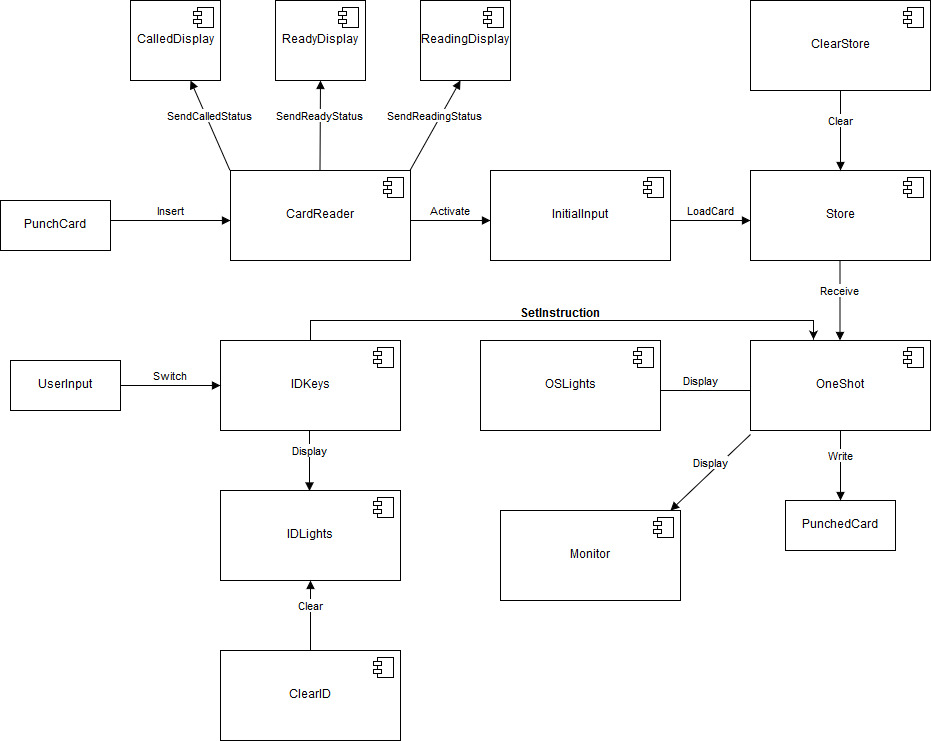
\includegraphics[width=\linewidth]{images/deuce-uml}
	\caption{UML diagram describing the system architecture.}
	\label{fig:uml}
\end{figure}

To help visualise the instruction processing of the emulator more clearly, a UML diagram was created in the early stages of design, shown in Figure \ref{fig:uml}. The diagram shows the two forms of input a user can use to provide the emulator with data: either using a pre-written punch card, or the input switches on the console. If a punch card is entered, the card will be read in and the console will show the status of the card, either as being "Called", "Ready" or as "Being read". After the card has been read in, the Initial Input switch can be pressed to load the card into storage, so that program execution can begin. Storage can be cleared using the "clear store" switch.

For input via the Input Dynamiciser switches, the current state of the Input Dynamiciser will be displayed on the ID lights. These lights can be reset to 0 using the "Clear ID" switch. Each ID switch represents one bit of a 32-bit word. When the user wants to enter an instruction, they would press the "One Shot" switch to execute said instruction.

Regarding output, the DEUCE should display output on the Output Staticiser lights. These lights display the output of the last instruction executed as a 32-bit reverse binary word. The original DEUCE could also write output to punched cards or to the system's monitor. These features may not be implemented in this version of the DEUCE but it was important to show that these features were part of the original DEUCE architecture.

From using this diagram, the flow of program execution in the DEUCE can be seen. It identifies the key components of the DEUCE based on the functional requirements from Chapter 3.

\section{User Interface}
One of the key differences between the interface of the DEUCE emulator and the original DEUCE interface is the lack of hardware. Given that this project would be written entirely as software, one of they key challenges would be replicating the physical features of the DEUCE within software and representing them correctly to the user. To solve this problem, visual metaphors would need to be used to allow the user to feel as though they were using the original DEUCE.

The DEUCE is comprised of many switches and lights. It also features a dial to set the number of single shots to be executed in succession. While it is not possible to physically recreate these components, it is important to give the user correct feedback when operating them. To solve this challenge, it was decided that switches and lights would need to be animated properly to give the user good feedback on their actions.

Another large difference between a software-only DEUCE and a real DEUCE is the absence of a card reader and card punch. In the original DEUCE, a Hollerith card reader was used to read in pre-written programs and a card punch was used to physically print output on card. To replicate a card reader in a web application, a good solution would be to provide a file upload button and have users browse files to mimic inserting a program into the DEUCE. A better solution would be to use a web framework that supports "drag and drop" features, which would allow a user to "drop" a card into the card reader. 

For these reasons, it was necessary to select a web framework that would support these graphical needs.


%==================================================================================================================================
\chapter{Implementation}
This chapter discusses the implementation of the DEUCE emulator and how 
\section{Web framework choice}
\subsection{Angular}
\subsection{React}
\subsection{Vue.js}
\section{Front-end development}
\section{Back-end development}
\section{Guidance}
You can't talk about everything. Cover the high level first, then cover important, relevant or impressive details.

\section{General points}
These points apply to the whole dissertation, not just this chapter.

\subsection{Figures}
\emph{Always} refer to figures included, like Figure \ref{fig:relu}, in the body of the text. Include full, explanatory captions and make sure the figures look good on the page.
You may include multiple figures in one float, as in Figure \ref{fig:synthetic}, using \texttt{subcaption}, which is enabled in the template.



% Figures are important. Use them well.
\begin{figure}
    \centering
    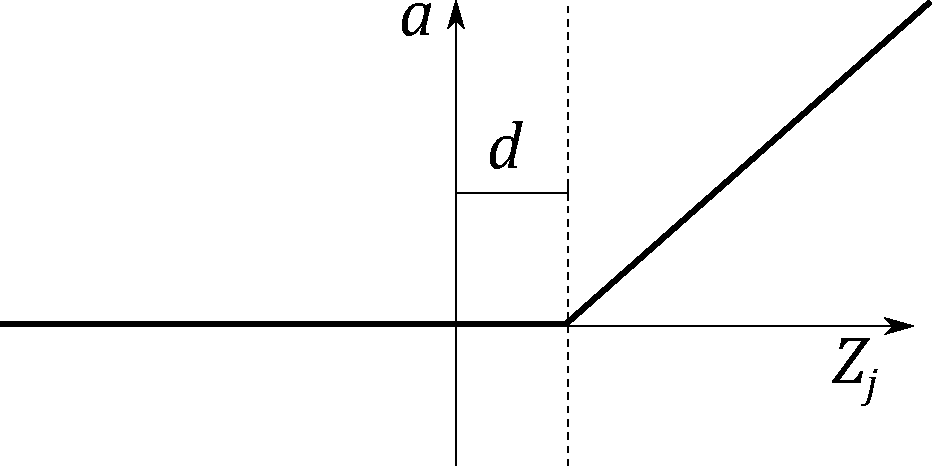
\includegraphics[width=0.5\linewidth]{images/relu.pdf}    

    \caption{In figure captions, explain what the reader is looking at: ``A schematic of the rectifying linear unit, where $a$ is the output amplitude,
    $d$ is a configurable dead-zone, and $Z_j$ is the input signal'', as well as why the reader is looking at this: 
    ``It is notable that there is no activation \emph{at all} below 0, which explains our initial results.'' 
    \textbf{Use vector image formats (.pdf) where possible}. Size figures appropriately, and do not make them over-large or too small to read.
    }

    % use the notation fig:name to cross reference a figure
    \label{fig:relu} 
\end{figure}


\begin{figure}
    \centering
    \begin{subfigure}[b]{0.45\textwidth}
        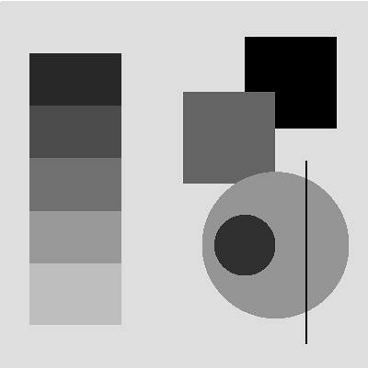
\includegraphics[width=\textwidth]{images/synthetic.png}
        \caption{Synthetic image, black on white.}
        \label{fig:syn1}
    \end{subfigure}
    ~ %add desired spacing between images, e. g. ~, \quad, \qquad, \hfill etc. 
      %(or a blank line to force the subfigure onto a new line)
    \begin{subfigure}[b]{0.45\textwidth}
        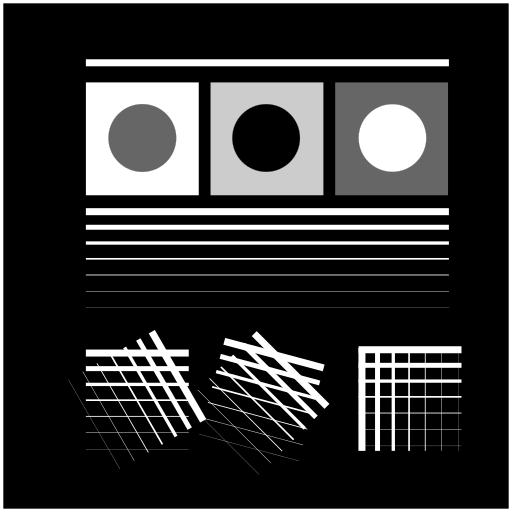
\includegraphics[width=\textwidth]{images/synthetic_2.png}
        \caption{Synthetic image, white on black.}
        \label{fig:syn2}
    \end{subfigure}
    ~ %add desired spacing between images, e. g. ~, \quad, \qquad, \hfill etc. 
    %(or a blank line to force the subfigure onto a new line)    
    \caption{Synthetic test images for edge detection algorithms. \subref{fig:syn1} shows various gray levels that require an adaptive algorithm. \subref{fig:syn2}
    shows more challenging edge detection tests that have crossing lines. Fusing these into full segments typically requires algorithms like the Hough transform.
    }\label{fig:synthetic}
\end{figure}

\clearpage

\subsection{Equations}

Equations should be typeset correctly and precisely. Make sure you get parenthesis sizing correct, and punctuate equations correctly 
(the comma is important and goes \textit{inside} the equation block). Explain any symbols used clearly if not defined earlier. 

For example, we might define:
\begin{equation}
    \hat{f}(\xi) = \frac{1}{2}\left[ \int_{-\infty}^{\infty} f(x) e^{2\pi i x \xi} \right],
\end{equation}    
where $\hat{f}(\xi)$ is the Fourier transform of the time domain signal $f(x)$.


\subsection{Tables}

If you need to include tables, like Table \ref{tab:operators}, use a tool like https://www.tablesgenerator.com/ to generate the table as it is
extremely tedious otherwise. 

\begin{table}[]
    \caption{The standard table of operators in Python, along with their functional equivalents from the \texttt{operator} package. Note that table
    captions go above the table, not below. Do not add additional rules/lines to tables. }\label{tab:operators}
    %\tt 
    \rowcolors{2}{}{gray!3}
    \begin{tabular}{@{}lll@{}}
    %\toprule
    \textbf{Operation}    & \textbf{Syntax}                & \textbf{Function}                            \\ %\midrule % optional rule for header
    Addition              & \texttt{a + b}                          & \texttt{add(a, b)}                                    \\
    Concatenation         & \texttt{seq1 + seq2}                    & \texttt{concat(seq1, seq2)}                           \\
    Containment Test      & \texttt{obj in seq}                     & \texttt{contains(seq, obj)}                           \\
    Division              & \texttt{a / b}                          & \texttt{div(a, b) }  \\
    Division              & \texttt{a / b}                          & \texttt{truediv(a, b) } \\
    Division              & \texttt{a // b}                         & \texttt{floordiv(a, b)}                               \\
    Bitwise And           & \texttt{a \& b}                         & \texttt{and\_(a, b)}                                  \\
    Bitwise Exclusive Or  & \texttt{a \textasciicircum b}           & \texttt{xor(a, b)}                                    \\
    Bitwise Inversion     & \texttt{$\sim$a}                        & \texttt{invert(a)}                                    \\
    Bitwise Or            & \texttt{a | b}                          & \texttt{or\_(a, b)}                                   \\
    Exponentiation        & \texttt{a ** b}                         & \texttt{pow(a, b)}                                    \\
    Identity              & \texttt{a is b}                         & \texttt{is\_(a, b)}                                   \\
    Identity              & \texttt{a is not b}                     & \texttt{is\_not(a, b)}                                \\
    Indexed Assignment    & \texttt{obj{[}k{]} = v}                 & \texttt{setitem(obj, k, v)}                           \\
    Indexed Deletion      & \texttt{del obj{[}k{]}}                 & \texttt{delitem(obj, k)}                              \\
    Indexing              & \texttt{obj{[}k{]}}                     & \texttt{getitem(obj, k)}                              \\
    Left Shift            & \texttt{a \textless{}\textless b}       & \texttt{lshift(a, b)}                                 \\
    Modulo                & \texttt{a \% b}                         & \texttt{mod(a, b)}                                    \\
    Multiplication        & \texttt{a * b}                          & \texttt{mul(a, b)}                                    \\
    Negation (Arithmetic) & \texttt{- a}                            & \texttt{neg(a)}                                       \\
    Negation (Logical)    & \texttt{not a}                          & \texttt{not\_(a)}                                     \\
    Positive              & \texttt{+ a}                            & \texttt{pos(a)}                                       \\
    Right Shift           & \texttt{a \textgreater{}\textgreater b} & \texttt{rshift(a, b)}                                 \\
    Sequence Repetition   & \texttt{seq * i}                        & \texttt{repeat(seq, i)}                               \\
    Slice Assignment      & \texttt{seq{[}i:j{]} = values}          & \texttt{setitem(seq, slice(i, j), values)}            \\
    Slice Deletion        & \texttt{del seq{[}i:j{]}}               & \texttt{delitem(seq, slice(i, j))}                    \\
    Slicing               & \texttt{seq{[}i:j{]}}                   & \texttt{getitem(seq, slice(i, j))}                    \\
    String Formatting     & \texttt{s \% obj}                       & \texttt{mod(s, obj)}                                  \\
    Subtraction           & \texttt{a - b}                          & \texttt{sub(a, b)}                                    \\
    Truth Test            & \texttt{obj}                            & \texttt{truth(obj)}                                   \\
    Ordering              & \texttt{a \textless b}                  & \texttt{lt(a, b)}                                     \\
    Ordering              & \texttt{a \textless{}= b}               & \texttt{le(a, b)}                                     \\
    % \bottomrule
    \end{tabular}
    \end{table}
\subsection{Code}

Avoid putting large blocks of code in the report (more than a page in one block, for example). Use syntax highlighting if possible, as in Listing \ref{lst:callahan}.

\begin{lstlisting}[language=python, float, caption={The algorithm for packing the $3\times 3$ outer-totalistic binary CA successor rule into a 
    $16\times 16\times 16\times 16$ 4 bit lookup table, running an equivalent, notionally 16-state $2\times 2$ CA.}, label=lst:callahan]
    def create_callahan_table(rule="b3s23"):
        """Generate the lookup table for the cells."""        
        s_table = np.zeros((16, 16, 16, 16), dtype=np.uint8)
        birth, survive = parse_rule(rule)

        # generate all 16 bit strings
        for iv in range(65536):
            bv = [(iv >> z) & 1 for z in range(16)]
            a, b, c, d, e, f, g, h, i, j, k, l, m, n, o, p = bv

            # compute next state of the inner 2x2
            nw = apply_rule(f, a, b, c, e, g, i, j, k)
            ne = apply_rule(g, b, c, d, f, h, j, k, l)
            sw = apply_rule(j, e, f, g, i, k, m, n, o)
            se = apply_rule(k, f, g, h, j, l, n, o, p)

            # compute the index of this 4x4
            nw_code = a | (b << 1) | (e << 2) | (f << 3)
            ne_code = c | (d << 1) | (g << 2) | (h << 3)
            sw_code = i | (j << 1) | (m << 2) | (n << 3)
            se_code = k | (l << 1) | (o << 2) | (p << 3)

            # compute the state for the 2x2
            next_code = nw | (ne << 1) | (sw << 2) | (se << 3)

            # get the 4x4 index, and write into the table
            s_table[nw_code, ne_code, sw_code, se_code] = next_code

        return s_table

\end{lstlisting}

%==================================================================================================================================
\chapter{Evaluation} 
How good is your solution? How well did you solve the general problem, and what evidence do you have to support that?

\section{Comparison of features with original DEUCE}
\section{Guidance}
\begin{itemize}
    \item
        Ask specific questions that address the general problem.
    \item
        Answer them with precise evidence (graphs, numbers, statistical
        analysis, qualitative analysis).
    \item
        Be fair and be scientific.
    \item
        The key thing is to show that you know how to evaluate your work, not
        that your work is the most amazing product ever.
\end{itemize}

\section{Evidence}
Make sure you present your evidence well. Use appropriate visualisations, reporting techniques and statistical analysis, as appropriate.

If you visualise, follow the basic rules, as illustrated in Figure \ref{fig:boxplot}:
\begin{itemize}
\item Label everything correctly (axis, title, units).
\item Caption thoroughly.
\item Reference in text.
\item \textbf{Include appropriate display of uncertainty (e.g. error bars, Box plot)}
\item Minimize clutter.
\end{itemize}

See the file \texttt{guide\_to\_visualising.pdf} for further information and guidance.

\begin{figure}
    \centering
    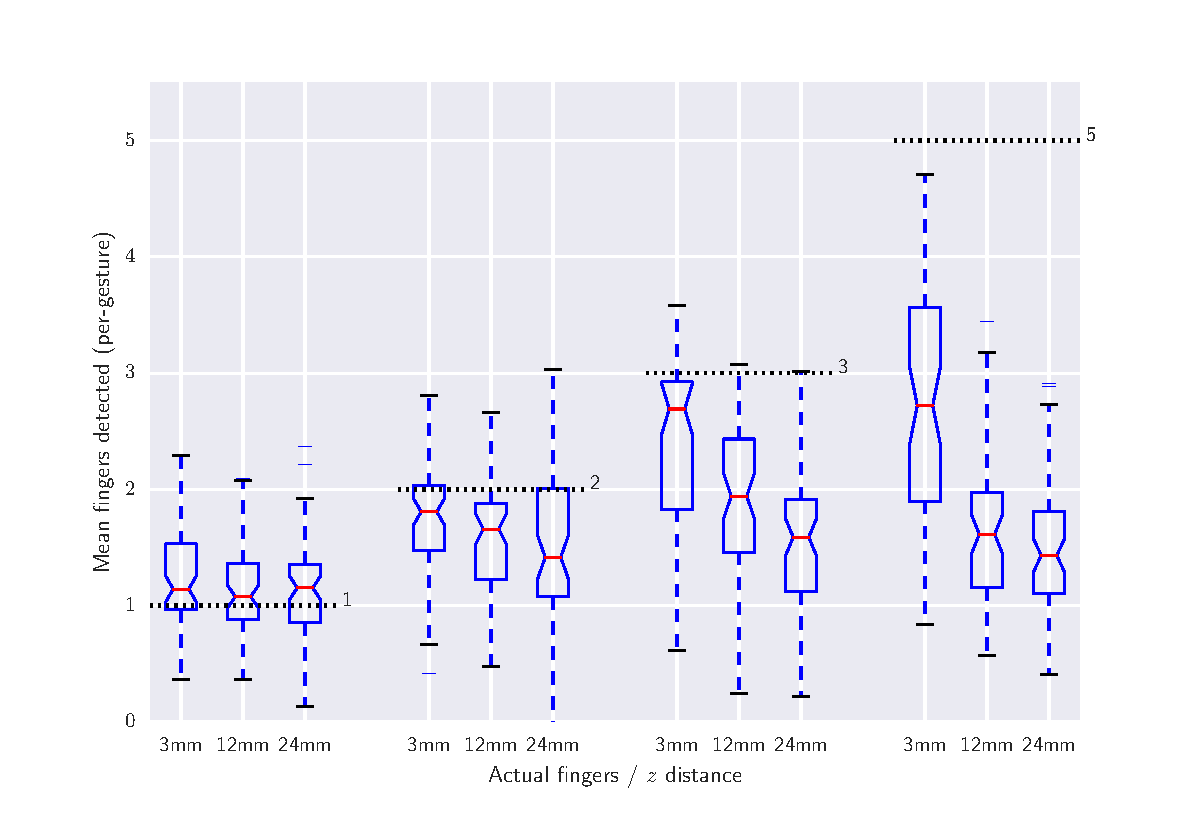
\includegraphics[width=1.0\linewidth]{images/boxplot_finger_distance.pdf}    

    \caption{Average number of fingers detected by the touch sensor at different heights above the surface, averaged over all gestures. Dashed lines indicate
    the true number of fingers present. The Box plots include bootstrapped uncertainty notches for the median. It is clear that the device is biased toward 
    undercounting fingers, particularly at higher $z$ distances.
    }

    % use the notation fig:name to cross reference a figure
    \label{fig:boxplot} 
\end{figure}


%==================================================================================================================================
\chapter{Conclusion}    
Summarise the whole project for a lazy reader who didn't read the rest (e.g. a prize-awarding committee).
\section{Guidance}
\begin{itemize}
    \item
        Summarise briefly and fairly.
    \item
        You should be addressing the general problem you introduced in the
        Introduction.        
    \item
        Include summary of concrete results (``the new compiler ran 2x
        faster'')
    \item
        Indicate what future work could be done, but remember: \textbf{you
        won't get credit for things you haven't done}.
\end{itemize}

%==================================================================================================================================
%
% 
%==================================================================================================================================
%  APPENDICES  

\begin{appendices}

\chapter{Appendices}

Typical inclusions in the appendices are:

\begin{itemize}
\item
  Copies of ethics approvals (required if obtained)
\item
  Copies of questionnaires etc. used to gather data from subjects.
\item
  Extensive tables or figures that are too bulky to fit in the main body of
  the report, particularly ones that are repetitive and summarised in the body.

\item Outline of the source code (e.g. directory structure), or other architecture documentation like class diagrams.

\item User manuals, and any guides to starting/running the software.

\end{itemize}

\textbf{Don't include your source code in the appendices}. It will be
submitted separately.

\end{appendices}

%==================================================================================================================================
%   BIBLIOGRAPHY   

% The bibliography style is abbrvnat
% The bibliography always appears last, after the appendices.

\bibliographystyle{abbrvnat}

\bibliography{l4proj}

\end{document}
